% Provenance (never printed): see sources/outline_sources.md (Year 3:
% stereographic projection; fold and fault analysis; palaeostress; balanced
% cross-sections). Brief: sources/book5/BRIEFS.md, ch. 8. Nets, pi-diagram and
% fault-slip data from figdata/bachelor-3/stereonet.py (Varden data invented,
% from figdata/shared/region.py); Fry plot from figdata/bachelor-3/fry.py.
% Exercise and problem values in the Book 5 scratch calculator calc/ch08.py.
% No real-world numbers: no ledger rows.
\chapter{Structural Analysis}\label{ch:b3:structural-analysis}

A geologist has measured two hundred bedding planes on the limbs of a fold
too large to be seen whole: its hinge lies under a forest, its limbs run for
kilometres. Each reading is a pair of numbers. Plotted as points on a circular
chart, the \omterm{def:b3:structural-analysis:stereo}{poles} of the planes fall along a single curve, a great circle, and
the \omterm{def:b3:structural-analysis:stereo}{pole} of that great circle is the axis of the fold, a line that nobody has
ever seen. This chapter builds the chart, the \omterm{def:b3:structural-analysis:stereo}{stereographic projection}, and
uses it, with the vector tools behind it, to find fold axes, to measure the
strain recorded by deformed objects, to recover the stress that drove a set of
faults, and to restore a deformed cross-section to its state before the
deformation.

\begin{recall}
Great and small circles of a sphere are in the Year 1 volume, in its chapter
on spherical astronomy; strike, dip, dip direction, trend and plunge in its
chapters on geological maps and cross-sections; the upward unit normal of a
plane of dip direction $\alpha$ and dip $\delta$, $\vec n = (\sin\delta
\sin\alpha, \sin\delta\cos\alpha, \cos\delta)$ in east, north and up
components, and the vector mean of a set of readings in its first chapter on
field and laboratory methods. Fold elements and classes, the hinge line of a
fold parallel to $\vec n_1\times\vec n_2$ and the interlimb angle
$\ang{180} - \arccos(\vec n_1\cdot\vec n_2)$, as well as Anderson's theory of
faulting, are in its chapter on faults, folds and fabrics; stress, the
principal stresses, the strain ellipse and simple shear in its chapter on
stress, strain and rheology; the rake of a slip vector (from the strike,
\ang{-90} for a normal fault, \ang{90} for a reverse fault, 0 sinistral and
\ang{180} dextral) and the P and T axes of a focal mechanism in its chapter on
the earthquake source. The balanced cross-section and the décollement are in
the Year 2 volume, in its chapter on the Alps. Least squares are in
\cref{sec:b3:seismology-imaging:inverse}; eigenvalues and eigenvectors of a
symmetric matrix are in the mathematics books.
\end{recall}

\section{The stereographic projection}\label{sec:b3:structural-analysis:stereo}

A geologist's data are orientations: the attitude of a bedding plane, a
fault, a foliation; the trend and plunge of a lineation, a fold hinge, a slip
direction. Each one is a direction through a point, with no position. To
compare hundreds of them, imagine them all moved to the centre of one sphere:
a line meets the lower half of the sphere at one point, a plane cuts it along
a half great circle. A chart of the lower hemisphere then shows lines as
points and planes as curves.

\begin{definition}[Stereographic projection, equal-angle net, equal-area projection, pole]\label{def:b3:structural-analysis:stereo}
Let a line through the centre $O$ of a sphere of radius $R$ meet the lower
hemisphere at $P$, at the angle $\theta = \ang{90} - p$ from the nadir, where
$p$ is the plunge of the line and $t$ its trend. The \emph{stereographic
projection}\index{stereographic projection} maps $P$ to the point where the
straight line from the zenith to $P$ crosses the horizontal plane through
$O$; that point lies at the distance $r$ from $O$ in the azimuth $t$. The
chart of the lower hemisphere drawn this way, with its grid of great and
small circles, is the \emph{equal-angle net}\index{equal-angle net} (or
Wulff net). The \emph{equal-area projection (of the sphere)}\index{equal-area
projection (of the sphere)} maps $P$ to the point at the distance $r =
R\sqrt2\sin(\theta/2)$ in the azimuth $t$; its net is the Schmidt net. The
\emph{pole}\index{pole (to a plane)} of a plane is its normal line, plotted as
a point: for a plane of dip direction $\alpha$ and dip $\delta$, the pole
trends $\alpha + \ang{180}$ and plunges $\ang{90} - \delta$.
\end{definition}

Both projections put a vertical line at the centre and a horizontal line on
the circle of radius $R$, the primitive. They differ in what they keep.

\begin{theorem}[The two projections]\label{thm:b3:structural-analysis:projections}
\begin{enumerate}[label=(\alph*)]
  \item The \omterm{def:b3:structural-analysis:stereo}{stereographic projection} places $P$ at $r = R\tan(\theta/2)$. It
        is conformal: at every point it stretches all directions by the same
        factor, $1/(2\cos^2(\theta/2))$, so that it keeps the angles between
        curves.
  \item The equal-area projection multiplies every area by the same factor,
        $1/2$: the area of a region of the net is half the area of the region
        of the hemisphere that it represents.
\end{enumerate}
\end{theorem}

\begin{proof}
(a) In the vertical plane through the zenith $Z$, the nadir and $P$
(first figure below), the arc from the nadir to $P$
subtends the angle $\theta$ at the centre, hence the inscribed angle
$\theta/2$ at $Z$, which is at the distance $R$ above $O$: $r =
R\tan(\theta/2)$. A small step $R\,\mathrm d\theta$ on the sphere towards the
nadir becomes $\mathrm dr = R\,\mathrm d\theta/(2\cos^2(\theta/2))$ on the
chart. The circle of points at the angle $\theta$ from the nadir has the
circumference $2\pi R\sin\theta$ and becomes a circle of circumference $2\pi
r$; the ratio is $\tan(\theta/2)/\sin\theta = 1/(2\cos^2(\theta/2))$, the same
as along the radius. A map that stretches equally in two perpendicular
directions stretches equally in all directions and keeps angles.

(b) The cap of the sphere within the angle $\theta$ of the nadir has the area
$2\pi R^2(1 - \cos\theta) = 4\pi R^2\sin^2(\theta/2)$; its image is the disc
of area $\pi r^2 = 2\pi R^2\sin^2(\theta/2)$, half of it. Both areas are
shared out evenly in azimuth, so the sector of the cap between two azimuths
and its image keep the ratio $1/2$, and so does the ring between two values
of $\theta$, the difference of two caps. Every region is a union of such
small ring sectors.
\end{proof}

The \omterm{def:b3:structural-analysis:stereo}{stereographic projection} also maps every circle of the sphere, great or
small, to a circle or a straight line on the chart; we admit this. It makes the
\omterm{def:b3:structural-analysis:stereo}{equal-angle net} easy to draw with compasses, and a small circle, the cone of
the lines at a fixed angle from an axis, keeps its shape. The equal-area
projection distorts shapes: a small circle becomes an oval, stretched
around the primitive. It is the projection on which a cloud of \omterm{def:b3:structural-analysis:stereo}{poles} can be
counted, since an equal area of the net holds an equal share of the
hemisphere's directions; structural geologists, and seismologists for their
focal mechanisms, use it for their data.

\begin{omfigure}
\begin{tikzpicture}[scale=1.0, >=stealth]
% (a) equal-angle: theta = 60 deg, R = 2 cm; r = 2 tan 30 = 1.155
\begin{scope}
\draw[thick] (0,0) circle (2);
\draw (-2.5,0) -- (2.5,0) node[right, font=\scriptsize] {plane};
\fill (0,2) circle (1.5pt) node[above, font=\scriptsize] {zenith $Z$};
\fill (0,-2) circle (1.5pt) node[below, font=\scriptsize] {nadir};
\fill (0,0) circle (1.2pt) node[above left, font=\scriptsize] {$O$};
\draw[dashed] (0,2) -- (0,-2);
\draw[omDef, thick] (0,0) -- (1.732,-1);
\fill[omDef] (1.732,-1) circle (1.5pt) node[below right, font=\scriptsize] {$P$};
\draw[omThm] (0,2) -- (1.732,-1);
\fill[omThm] (1.155,0) circle (1.5pt);
\node[omThm, font=\scriptsize, above right] at (1.155,0) {$P'$};
\draw (0,-0.6) arc[start angle=-90, end angle=-30, radius=0.6];
\node[font=\scriptsize] at (0.38,-0.85) {$\theta$};
\draw (0,1.2) arc[start angle=-90, end angle=-60, radius=0.8];
\node[font=\scriptsize] at (0.25,0.95) {$\theta/2$};
\draw[<->] (0,0.25) -- (1.155,0.25);
\node[font=\scriptsize, above] at (0.58,0.25) {$r$};
\node[font=\small] at (0,-3.0) {(a) equal-angle};
\end{scope}
% (b) equal-area: chord from nadir to P = 2R sin(theta/2) = 2
\begin{scope}[xshift=6.6cm]
\draw[thick] (0,0) circle (2);
\draw (-2.5,0) -- (2.5,0);
\draw (-2.5,-2) -- (2.5,-2) node[right, font=\scriptsize] {tangent plane};
\fill (0,-2) circle (1.5pt) node[below left, font=\scriptsize] {nadir};
\fill (0,0) circle (1.2pt) node[above left, font=\scriptsize] {$O$};
\draw[dashed] (0,2) -- (0,-2);
\draw[omDef, thick] (0,0) -- (1.732,-1);
\fill[omDef] (1.732,-1) circle (1.5pt) node[above right, font=\scriptsize] {$P$};
\draw[omThm] (0,-2) -- (1.732,-1);
\draw[omThm, dashed] (1.732,-1) arc[start angle=30, end angle=0, radius=2];
\fill[omThm] (2,-2) circle (1.5pt);
\node[omThm, font=\scriptsize, below] at (2,-2.05) {$2R\sin(\theta/2)$};
\draw (0,-0.6) arc[start angle=-90, end angle=-30, radius=0.6];
\node[font=\scriptsize] at (0.38,-0.85) {$\theta$};
\node[font=\small] at (0,-3.0) {(b) equal-area};
\end{scope}
\end{tikzpicture}

\par\smallskip{\small The two projections, in the vertical plane through the
line $OP$. (a) The \omterm{def:b3:structural-analysis:stereo}{stereographic projection} sends $P$ to $P'$, where the line
from the zenith crosses the horizontal plane: the angle at $Z$ is
$\theta/2$, so $r = R\tan(\theta/2)$. (b) The equal-area projection carries
$P$, around the nadir, onto the tangent plane at the distance $2R\sin(\theta/2)$
of the chord; the chart is then scaled by $1/\sqrt2$ so that the horizontal
lines fall on a primitive of radius $R$.}\label{fig:b3:structural-analysis:geometry}
\end{omfigure}

\begin{omfigure}
\begin{tikzpicture}
\begin{groupplot}[group style={group size=2 by 1, horizontal sep=0.8cm},
  width=0.5\linewidth, height=0.5\linewidth, axis equal image, hide axis,
  xmin=-1.15, xmax=1.15, ymin=-1.15, ymax=1.15, unbounded coords=jump,
  title style={font=\small}]
\nextgroupplot[title={(a) equal-angle (Wulff) net}]
% computed in figdata/bachelor-3/stereonet.py
\addplot[gray!75, very thin] table[x=x, y=y] {figdata/out/bachelor-3-stereonet-wulff.dat};
\addplot[gray!75, very thin] coordinates {(-1,0) (1,0)};
\addplot[black, thick, domain=0:360, samples=181] ({cos(x)}, {sin(x)});
\node[font=\scriptsize, above] at (axis cs:0,1.0) {N};
\nextgroupplot[title={(b) equal-area (Schmidt) net}]
\addplot[gray!75, very thin] table[x=x, y=y] {figdata/out/bachelor-3-stereonet-schmidt.dat};
\addplot[gray!75, very thin] coordinates {(-1,0) (1,0)};
\addplot[black, thick, domain=0:360, samples=181] ({cos(x)}, {sin(x)});
\node[font=\scriptsize, above] at (axis cs:0,1.0) {N};
\end{groupplot}
\end{tikzpicture}

\par\smallskip{\small The two nets, drawn from the formulas of the theorem
above: great circles of the planes striking north--south and dipping every
\ang{10} east and west, and small circles every \ang{10} about the
north--south axis. On the \omterm{def:b3:structural-analysis:stereo}{equal-angle net} the small circles are circles; on
the equal-area net they are ovals, but equal areas hold equal shares of the
directions.}\label{fig:b3:structural-analysis:nets}
\end{omfigure}

\paragraph{Planes, lines and angles.}
A plane of dip direction $\alpha$ and dip $\delta$ cuts the lower hemisphere
along a half great circle. Its ends lie on the primitive at the two ends of
the strike; its middle is the line of steepest dip, which plunges $\delta$
towards $\alpha$; and its \omterm{def:b3:structural-analysis:stereo}{pole} lies \ang{90} from every point of it, in the
azimuth $\alpha + \ang{180}$. A line in the plane is a point on the great
circle. To plot data, a transparent overlay is laid on the net and turned
about the centre until the data's strike lies along the net's north--south
diameter; the great circle of the right dip is then traced, and the overlay is
turned back. The angle between two lines is measured along the great circle
through both points, counting the small-circle divisions it crosses, after
turning the overlay until both points lie on one great circle of the net. The
angle between two planes is the angle between their \omterm{def:b3:structural-analysis:stereo}{poles}, or its supplement.
A computer does the same with vectors: the angle between two lines of unit
vectors $\vec u$ and $\vec v$ is $\arccos|\vec u\cdot\vec v|$.

\begin{method}[Rotating data about an axis]\label{met:b3:structural-analysis:rotation}
To undo a tilt, for instance to bring a bed back to the horizontal with the
lineations that it carries, or to restore a palaeomagnetic direction measured
in tilted strata (\cref{ch:b3:palaeomagnetism}):
\begin{enumerate}
  \item Choose the axis of rotation: for a tilted bed, its strike line,
        horizontal; the angle is the dip, in the sense that brings the bed up.
  \item On the net, turn the overlay until the axis lies along the
        north--south diameter, where the small circles are the cones about
        it.
  \item Move every point along its small circle by the angle of rotation,
        counted on the great circles. A point that would leave the lower
        hemisphere reappears at the opposite end of its small circle, in the
        opposite azimuth.
  \item Turn the overlay back. With vectors, the rotation of $\vec v$ by the
        angle $\omega$ about the unit axis $\vec k$ is $\vec v' = \vec v
        \cos\omega + (\vec k\times\vec v)\sin\omega + \vec k(\vec k\cdot\vec
        v)(1 - \cos\omega)$.
\end{enumerate}
\end{method}

\section{Fold analysis}\label{sec:b3:structural-analysis:folds}

A cylindrical fold is generated by a straight line, the fold axis, moved
parallel to itself. Every plane tangent to the folded surface contains the
axis, so every normal to the surface is perpendicular to the axis: all the
\omterm{def:b3:structural-analysis:stereo}{poles} lie on the great circle of the plane perpendicular to the axis.

\begin{definition}[Pi-diagram, beta-axis]\label{def:b3:structural-analysis:pi}
The \emph{pi-diagram}\index{pi-diagram} of a fold is the plot of the \omterm{def:b3:structural-analysis:stereo}{poles} of
the planes measured on its folded surface. For a cylindrical fold they fall on
a great circle, the $\pi$-girdle; the \omterm{def:b3:structural-analysis:stereo}{pole} of the girdle is the
\emph{beta-axis}\index{beta-axis}, the estimate of the fold axis given by the
measurements.
\end{definition}

With two limbs only, the \omterm{def:b3:structural-analysis:pi}{beta-axis} is the cross product of their normals, as
the Year 1 volume showed for the hinge line. With two hundred scattered
readings, a best fit is needed. The vector mean, which served for the readings
of one plane, will not do: the \omterm{def:b3:structural-analysis:stereo}{poles} of a girdle point every way along it, and
their mean says little about the circle they lie on.

\begin{definition}[Orientation tensor]\label{def:b3:structural-analysis:orientation-tensor}
The \emph{orientation tensor}\index{orientation tensor} of $N$ unit vectors
$\vec p_1, \dots, \vec p_N$ is the symmetric matrix
\[
  T = \frac1N\sum_{i=1}^N \vec p_i\,\vec p_i^{\mathsf T},
  \qquad T_{jk} = \frac1N\sum_i p_{ij}\,p_{ik} .
\]
It does not change when a vector is replaced by its opposite, so it suits
axes and \omterm{def:b3:structural-analysis:stereo}{poles}, which have no sense. Its eigenvalues $\lambda_1 \ge \lambda_2
\ge \lambda_3 \ge 0$ add up to its trace, $1$.
\end{definition}

\begin{theorem}[Cluster and girdle from the orientation tensor]\label{thm:b3:structural-analysis:tensor}
For any unit vector $\vec u$,
\[
  \frac1N\sum_{i=1}^N (\vec p_i\cdot\vec u)^2 = \vec u^{\mathsf T}T\,\vec u ,
\]
which takes its smallest value, $\lambda_3$, when $\vec u$ is the eigenvector
$\vec e_3$ of the smallest eigenvalue, and its largest, $\lambda_1$, along the
eigenvector $\vec e_1$. Since $\vec p_i\cdot\vec u$ is the sine of the angle
between $\vec p_i$ and the plane perpendicular to $\vec u$, the great circle
perpendicular to $\vec e_3$ is the girdle that minimises the sum of the squared
sines of the distances of the \omterm{def:b3:structural-analysis:stereo}{poles} to it, and $\sqrt{\lambda_3}$ is their
root-mean-square sine. The axis $\vec e_1$ is the line closest to the vectors,
the mean axis of a cluster.
\end{theorem}

\begin{proof}
$(\vec p_i\cdot\vec u)^2 = \vec u^{\mathsf T}\vec p_i\,\vec p_i^{\mathsf T}\vec
u$; average over $i$. The matrix $T$ is symmetric, so it has an orthonormal
basis of eigenvectors, in which $\vec u = \sum_k u_k\vec e_k$ with $\sum_k
u_k^2 = 1$ and $\vec u^{\mathsf T}T\vec u = \sum_k\lambda_k u_k^2$. This is a
weighted mean of the eigenvalues, with weights $u_k^2$ that add up to 1: it
lies between $\lambda_3$ and $\lambda_1$ and reaches them for $\vec u = \vec
e_3$ and $\vec e_1$.
\end{proof}

The eigenvalues describe the shape of the data. A cluster has $\lambda_1$ near
1 and the other two small; a girdle has $\lambda_3$ near 0, the \omterm{def:b3:structural-analysis:stereo}{poles} being
spread along the circle so that $\lambda_1$ and $\lambda_2$ share the rest;
uniformly scattered vectors give three eigenvalues near $1/3$. A fold is
cylindrical, within the precision of the readings, when $\sqrt{\lambda_3}$ is
no larger than the scatter of repeated readings of one plane. A conical fold,
or two generations of folds, spread the \omterm{def:b3:structural-analysis:stereo}{poles} away from any one great circle
and raise $\lambda_3$.

The figure below plots twelve readings from the two limbs of the Varden
anticline, the series' invented fold (\cref{pb:b3:structural-analysis:1}
computes its axis). The \omterm{def:b3:structural-analysis:stereo}{poles} of the gentle limbs cluster near the centre of
the net in two groups, which together define a girdle running almost
east--west; the \omterm{def:b3:structural-analysis:pi}{beta-axis} lies on the primitive, almost due north. The mean
planes of the two limbs, drawn as great circles, cross at the same point:
the \omterm{def:b3:structural-analysis:pi}{beta-axis} is the line common to all the limbs.

\begin{omfigure}
\begin{tikzpicture}
\begin{groupplot}[group style={group size=2 by 1, horizontal sep=1.0cm},
  width=0.5\linewidth, height=0.5\linewidth, axis equal image,
  unbounded coords=jump, title style={font=\small}]
\nextgroupplot[hide axis, xmin=-1.15, xmax=1.15, ymin=-1.15, ymax=1.15,
  title={(a) the lower hemisphere}]
% computed in figdata/bachelor-3/stereonet.py (Varden readings invented)
\addplot[gray!35, very thin] table[x=x, y=y] {figdata/out/bachelor-3-stereonet-schmidt.dat};
\addplot[black, thick, domain=0:360, samples=181] ({cos(x)}, {sin(x)});
\addplot[gray, densely dashed] table[x=x, y=y] {figdata/out/bachelor-3-stereonet-limbs.dat};
\addplot[omDef, thick] table[x=x, y=y] {figdata/out/bachelor-3-stereonet-girdle.dat};
\addplot[only marks, mark=*, mark size=1.2pt] table[x=x, y=y] {figdata/out/bachelor-3-stereonet-poles.dat};
\addplot[only marks, mark=triangle*, mark size=3pt, omThm] table[x=x, y=y] {figdata/out/bachelor-3-stereonet-beta.dat};
\node[font=\scriptsize, above] at (axis cs:0,1.02) {N};
\node[omThm, font=\scriptsize, right] at (axis cs:0.06,0.88) {$\beta$};
\draw[gray] (axis cs:-0.3,-0.3) rectangle (axis cs:0.3,0.3);
\nextgroupplot[xmin=-0.3, xmax=0.3, ymin=-0.3, ymax=0.3, title={(b) the centre, enlarged},
  xtick=\empty, ytick=\empty]
\addplot[gray!35, very thin] table[x=x, y=y] {figdata/out/bachelor-3-stereonet-schmidt.dat};
\addplot[omDef, thick] table[x=x, y=y] {figdata/out/bachelor-3-stereonet-girdle.dat};
\addplot[only marks, mark=*, mark size=1.5pt] table[x=x, y=y] {figdata/out/bachelor-3-stereonet-poles.dat};
\node[font=\scriptsize, align=center] at (axis cs:0.16,0.09) {poles of the\\ west limb};
\node[font=\scriptsize, align=center] at (axis cs:-0.16,0.09) {poles of the\\ east limb};
\node[omDef, font=\scriptsize] at (axis cs:0.17,-0.06) {$\pi$-girdle};
\end{groupplot}
\end{tikzpicture}

\par\smallskip{\small \omterm{def:b3:structural-analysis:pi}{Pi-diagram} of the Varden anticline on the equal-area
net, lower hemisphere: the \omterm{def:b3:structural-analysis:stereo}{poles} of twelve bedding readings (dots), the
best-fit girdle from the \omterm{def:b3:structural-analysis:orientation-tensor}{orientation tensor} (blue), the great circles of the
two mean limbs (dashed) and the \omterm{def:b3:structural-analysis:pi}{beta-axis} (triangle), where all three great
circles meet. A bed dipping east has its \omterm{def:b3:structural-analysis:stereo}{pole} to the west of the
centre.}\label{fig:b3:structural-analysis:pi}
\end{omfigure}

\section{Finite strain analysis}\label{sec:b3:structural-analysis:strain}

A deformed rock records its strain when it contains objects whose original
shape, or whose original arrangement, is known: round ooids and reduction
spots, fossils of known symmetry, pebbles, or simply the centres of grains
that were once evenly spaced.

\begin{definition}[Finite strain analysis, Fry method]\label{def:b3:structural-analysis:strain-analysis}
\emph{Finite strain analysis}\index{finite strain analysis} is the measurement
of the strain ellipse, or ellipsoid, that a rock has undergone, from the
shapes, orientations or spacings of objects whose state before the
deformation is known. In the \emph{Fry method}\index{Fry method}, the vector
from the centre of every object to the centre of every other is plotted from
one common origin; when the centres were spread with a minimum spacing and no
preferred direction, the empty region around the origin is an ellipse of the
shape and orientation of the strain ellipse.
\end{definition}

\begin{proposition}[The Fry void]\label{prop:b3:structural-analysis:fry}
If a homogeneous strain maps every vector $\vec d$ to $F\vec d$, and no two
centres were closer than $d_0$ before the strain, then after it the region
around the origin of the Fry plot that is free of points contains the ellipse
$\{F\vec d : |\vec d| < d_0\}$, of semi-axes $S_1d_0$ and $S_2d_0$ along the
principal directions of the strain.
\end{proposition}

\begin{proof}
A homogeneous strain moves every point by the same linear map, plus a
translation, so the difference of two centres becomes $F\vec d$. Before the
strain no difference lay in the disc of radius $d_0$; afterwards none lies in
its image, which is the strain ellipse of the Year 1 volume scaled by $d_0$.
\end{proof}

In practice the centres are not all at the minimum spacing, and the void is
read as the inner edge of the densest ring of points; its ratio estimates the
strain ratio $R_s = S_1/S_2$ slightly low. The figure below makes the test on
an invented thin section, strained to $R_s = 2$ with the long axis at
\ang{30} from the horizontal: the ellipse fitted to the edge of the void gives
$R_s = 1.9$ and \ang{30}. When the objects themselves are measured, initially
round ones become ellipses of the axial ratio $R_s$ exactly; initially
elliptical ones, with random orientations, end with ratios $R_f$ scattered
about $R_s$, the largest when their long axes started parallel to the
stretching direction, and their final orientations $\varphi$ gather around
it. The plot of $R_f$ against $\varphi$, read with tables or a computer,
separates the strain from the original shapes.

\begin{omfigure}
\begin{tikzpicture}
\begin{groupplot}[group style={group size=2 by 1, horizontal sep=1.2cm},
  width=0.5\linewidth, height=0.5\linewidth, axis equal image,
  title style={font=\small}, tick label style={font=\scriptsize}]
\nextgroupplot[xmin=-10, xmax=10, ymin=-10, ymax=10, title={(a) grain centres after the strain}]
% computed in figdata/bachelor-3/fry.py (invented population)
\addplot[only marks, mark=o, mark size=1.6pt, black] table[x=x, y=y] {figdata/out/bachelor-3-fry-points.dat};
\nextgroupplot[xmin=-2.6, xmax=2.6, ymin=-2.6, ymax=2.6, title={(b) Fry plot}]
\addplot[only marks, mark=*, mark size=0.5pt, black] table[x=x, y=y] {figdata/out/bachelor-3-fry-fry.dat};
\addplot[omThm, thick] table[x=x, y=y] {figdata/out/bachelor-3-fry-fit.dat};
\end{groupplot}
\end{tikzpicture}

\par\smallskip{\small The \omterm{def:b3:structural-analysis:strain-analysis}{Fry method} on an invented population of grain
centres, laid with a minimum spacing of 1 and then strained to $R_s = 2$,
long axis at \ang{30} anticlockwise from the horizontal, area kept. (a) The
centres, in which the eye hardly sees the strain. (b) The vectors between all
pairs of centres closer than 2.6: the empty centre is the strain ellipse. The
red ellipse is fitted to the nearest point in each of 36 sectors: ratio 1.9,
long axis at \ang{30}.}\label{fig:b3:structural-analysis:fry}
\end{omfigure}

In three dimensions the strain ellipsoid has the principal stretches $X \ge Y
\ge Z$. Its shape is plotted on the Flinn diagram, with $a = X/Y$ against $b =
Y/Z$ and the parameter
\[
  k = \frac{a - 1}{b - 1} .
\]
On the line $k = 1$, which holds plane strain at constant volume ($Y = 1$,
$X = 1/Z$, so $a = b$), the ellipsoid is neither cigar nor pancake. Above it,
$k > 1$, the ellipsoid is prolate, stretched in one direction by a
constriction: rocks deformed this way grow a strong lineation. Below, $k < 1$,
it is oblate, flattened, and the rock grows a strong foliation.

\begin{omfigure}
\begin{tikzpicture}[scale=1.0, >=stealth]
\draw[->] (0,0) -- (5.4,0) node[right, font=\scriptsize] {$b = Y/Z$};
\draw[->] (0,0) -- (0,4.6) node[above, font=\scriptsize] {$a = X/Y$};
\foreach \v/\l in {0/1, 1.5/2, 3/3, 4.5/4} {
  \draw (\v,0) -- (\v,-0.08) node[below, font=\scriptsize] {\l};
  \draw (0,\v) -- (-0.08,\v) node[left, font=\scriptsize] {\l};
}
\draw[omDef, thick] (0,0) -- (4.5,4.5) node[right, font=\scriptsize, align=left] {$k = 1$\\ plane strain};
\node[font=\scriptsize, align=center] at (1.3,3.6) {constriction\\ $k > 1$, prolate};
\node[font=\scriptsize, align=center] at (4.3,1.1) {flattening\\ $k < 1$, oblate};
% shapes
\draw[fill=omLithLime] (0.9,2.75) ellipse (0.55 and 0.12);
\draw[fill=omLithLime] (4.3,2.1) ellipse (0.45 and 0.22);
\end{tikzpicture}

\par\smallskip{\small The Flinn diagram of strain ellipsoids. The undeformed
state is the origin, $a = b = 1$; the cigar-shaped ellipsoids of constriction
lie towards the vertical axis, the pancakes of flattening towards the
horizontal one.}\label{fig:b3:structural-analysis:flinn}
\end{omfigure}

\section{Palaeostress}\label{sec:b3:structural-analysis:palaeostress}

Anderson's theory says on which planes new faults form, and that they slip
perpendicular to $\sigma_2$. Most faults, though, are older weaknesses
reactivated in a stress field that they did not choose, and they slip
obliquely. Their slip directions, read on the striations of the fault
surfaces, still record the stress, if each fault slips the way the stress
pushes it.

\begin{definition}[Palaeostress, Wallace--Bott hypothesis, stress ratio, fault-slip inversion]\label{def:b3:structural-analysis:palaeostress}
\emph{Palaeostress}\index{palaeostress} is the state of stress that acted in
a rock in the past, as far as it can be deduced from the structures it left:
in practice, the directions of the principal stresses and the
\emph{stress ratio}\index{stress ratio}
\[
  \Phi = \frac{\sigma_2 - \sigma_3}{\sigma_1 - \sigma_3}, \qquad 0 \le \Phi
  \le 1 .
\]
The \emph{Wallace--Bott hypothesis}\index{Wallace--Bott hypothesis} states
that a fault slips parallel to the shear stress resolved on its plane by a
uniform stress, each fault independently. A \emph{fault-slip
inversion}\index{fault-slip inversion} is the search for the principal
directions and the stress ratio whose predicted slip directions best fit a set
of measured faults and striations.
\end{definition}

\begin{theorem}[Slip direction on a plane]\label{thm:b3:structural-analysis:wallace-bott}
Let $S$ be the stress tensor, compressions counted positive, and $\vec n$ the
upward unit normal of a fault. Write
\[
  \vec\tau = S\vec n - (\vec n\cdot S\vec n)\,\vec n .
\]
Under the \omterm{def:b3:structural-analysis:palaeostress}{Wallace--Bott hypothesis} the hanging wall slips relative to the
footwall along $-\vec\tau$, the shear traction that it exerts on the
footwall. Moreover:
\begin{enumerate}[label=(\alph*)]
  \item the direction of $\vec\tau$ is unchanged when $S$ is replaced by $aS +
        bI$ with $a > 0$; it therefore depends only on the principal
        directions and on $\Phi$, and the reduced tensor $S' =
        \mathrm{diag}(1, \Phi, 0)$ in the principal frame $(\vec e_1, \vec
        e_2, \vec e_3)$ predicts the same slip as $S$;
  \item if $\vec n$ is perpendicular to one principal direction, the slip is
        perpendicular to it too;
  \item with $n_k = \vec n\cdot\vec e_k$, the direction is that of $\vec\tau'
        = \vec\tau_0 + \Phi\,\vec\tau_1$, linear in $\Phi$, where $\vec\tau_0
        = n_1(\vec e_1 - n_1\vec n)$ and $\vec\tau_1 = n_2(\vec e_2 - n_2\vec
        n)$.
\end{enumerate}
\end{theorem}

\begin{proof}
With compressions positive, the hanging wall pushes on the footwall, across
the plane of normal $\vec n$ pointing into the hanging wall, with the
traction $-S\vec n$; its part along the plane is $-\vec\tau$. When the
fault slips, the hanging wall moves the way it drags the footwall, along
$-\vec\tau$. (Check: with $\sigma_1$ vertical, $S = \sigma_1\vec e_z\vec
e_z^{\mathsf T}$ and $-\vec\tau = -\sigma_1\cos\delta\,(\vec e_z -
\cos\delta\,\vec n)$ points down the dip: a normal fault.)
(a) $(aS + bI)\vec n - (\vec n\cdot(aS + bI)\vec n)\vec n = a\vec\tau + b(\vec
n - \vec n) = a\vec\tau$. Writing $\sigma_k = \sigma_3 + (\sigma_1 -
\sigma_3)s_k$ with $s = (1, \Phi, 0)$ gives $S = \sigma_3 I + (\sigma_1 -
\sigma_3)S'$.
(b) $S\vec n = \sum_k\sigma_kn_k\vec e_k$; if $n_j = 0$, neither $S\vec n$
nor $\vec n$ has a component along $\vec e_j$, and neither has $\vec\tau$.
(c) $S'\vec n = n_1\vec e_1 + \Phi n_2\vec e_2$ and $\vec n\cdot S'\vec n =
n_1^2 + \Phi n_2^2$; collect the terms with and without $\Phi$.
\end{proof}

Part (b) is Anderson's case: a fault that contains $\sigma_2$ slips
perpendicular to it, whatever $\Phi$, so that it says nothing of the \omterm{def:b3:structural-analysis:palaeostress}{stress
ratio}. Part (c) turns a measured slip into $\Phi$. Let $\vec u$ be the unit
slip vector of the hanging wall, from the rake, and $\vec w = \vec n\times\vec
u$ the direction in the plane perpendicular to it. The predicted slip is
parallel to $\vec u$ when $(\vec\tau_0 + \Phi\vec\tau_1)\cdot\vec w = 0$, and
since $\vec n\cdot\vec w = 0$,
\[
  \Phi = -\frac{n_1\,(\vec e_1\cdot\vec w)}{n_2\,(\vec e_2\cdot\vec w)} ,
\]
provided the predicted slip then points along $+\vec u$ and not $-\vec u$.

When the principal directions are not known, each fault gives one equation,
the angle of its slip within its plane, for four unknowns: three angles that
orient the principal axes, and $\Phi$. Four faults of different attitudes are
the minimum, and a few tens are usual. The inversion minimises the sum of the
squared angles between the measured and the predicted slips, by least squares
on a grid or by iteration as in \cref{sec:b3:seismology-imaging:inverse}.
Faults that do not fit form a second population, perhaps of another age.

The figure below shows five faults of the Varden Hills: the main normal fault
and four smaller ones, all with normal slip. A grid search over $\Phi$ and the
trend of $\sigma_3$, with $\sigma_1$ vertical, fits all five within a quarter
of a degree, with $\sigma_3$ horizontal towards \ang{120}.

\begin{omfigure}
\begin{tikzpicture}
\begin{axis}[width=0.56\linewidth, height=0.56\linewidth, axis equal image,
  hide axis, xmin=-1.15, xmax=1.15, ymin=-1.15, ymax=1.15, unbounded coords=jump]
% computed in figdata/bachelor-3/stereonet.py (Varden faults invented)
\addplot[gray!35, very thin] table[x=x, y=y] {figdata/out/bachelor-3-stereonet-schmidt.dat};
\addplot[black, thick, domain=0:360, samples=181] ({cos(x)}, {sin(x)});
\addplot[omDef, thick] table[x=x, y=y] {figdata/out/bachelor-3-stereonet-faults.dat};
\addplot[only marks, mark=*, mark size=1.8pt, omDef] table[x=x, y=y] {figdata/out/bachelor-3-stereonet-slips.dat};
\addplot[only marks, mark=square*, mark size=2.6pt, omThm] table[x=x, y=y] {figdata/out/bachelor-3-stereonet-s1.dat};
\addplot[only marks, mark=diamond*, mark size=3pt, omProp] table[x=x, y=y] {figdata/out/bachelor-3-stereonet-s2.dat};
\addplot[only marks, mark=triangle*, mark size=3pt, omMeth] table[x=x, y=y] {figdata/out/bachelor-3-stereonet-s3.dat};
\node[font=\scriptsize, above] at (axis cs:0,1.02) {N};
\node[omThm, font=\scriptsize, above left] at (axis cs:0,0) {$\sigma_1$};
\node[omProp, font=\scriptsize, above right] at (axis cs:0.5,0.87) {$\sigma_2$};
\node[omMeth, font=\scriptsize, below right] at (axis cs:0.87,-0.5) {$\sigma_3$};
\end{axis}
\end{tikzpicture}

\par\smallskip{\small Fault-slip data of the Varden Hills on the equal-area
net, lower hemisphere: five fault planes (great circles) with the slip
direction of each hanging wall (dots), and the principal stresses of the
best-fitting stress: $\sigma_1$ vertical (square), $\sigma_2$ and $\sigma_3$
horizontal (diamonds and triangles, at both ends of each axis). The main
fault, dipping \ang{60} towards \ang{120}, contains $\sigma_2$ and slips
straight down its dip; the others slip
obliquely.}\label{fig:b3:structural-analysis:faults}
\end{omfigure}

The P and T axes of the Year 1 volume are not the principal stresses. They are
built from the fault plane and the slip alone, at \ang{45} from the plane in
the plane that contains the slip and the normal; a new fault, in rock with an
angle of friction near \ang{30}, makes about \ang{30} with $\sigma_1$, and a
reactivated one any angle. One mechanism gives the P and T axes; only many
faults of different attitudes, inverted together, give the stress. The
hypothesis itself has limits: the stress may vary from fault to fault, blocks
may rotate, and faults that meet hinder each other's slip.

\section{Restoring a cross-section}\label{sec:b3:structural-analysis:restoration}

A cross-section is an interpretation: between the surface and the boreholes,
the geologist draws what is likely. The Year 2 volume, in its chapter on the
Alps, called a section balanced when it can be returned to an undeformed state
with the lengths of the beds and the areas of the units conserved, folds and
thrusts rooting on a décollement. Restoring is the test.

\begin{definition}[Section restoration, pin line, kink-band method]\label{def:b3:structural-analysis:restoration}
\emph{Section restoration}\index{section restoration} undoes, on a
cross-section drawn parallel to the direction of tectonic transport, the
deformation it shows, event by event in the reverse order, keeping the
lengths of the beds and the areas of the units in the plane of the section.
A \emph{pin line}\index{pin line} is a line across the beds, placed where they
did not slip along each other (in the undeformed foreland, or on the axial
surface of a symmetric fold), which is taken to be perpendicular to the beds
in the restored section; lengths are measured from it. In the
\emph{kink-band method}\index{kink-band method} the folds are drawn as straight
limbs of constant bed thickness joined at sharp hinges, whose axial surfaces
bisect the angle between the limbs; each bed is then a broken line, whose
length is the sum of its straight segments.
\end{definition}

A bed folded into straight limbs dipping $\delta$ either way, over the
horizontal distance $L$, has the length $L/\cos\delta$: its shortening is
$S = L(1/\cos\delta - 1)$, the relative change of length $\cos\delta - 1$.
Areas give the other half of the balance.

\begin{proposition}[Depth to detachment]\label{prop:b3:structural-analysis:detachment}
Let a layer at the height $h$ above a horizontal detachment be shortened by $S$
in the plane of a section, and let the rock between it and the detachment
keep its area, with no material crossing the ends of the section. Then the
area $A$ by which the folded layer stands above its original level satisfies
\[
  A = S\,h , \qquad\text{so that}\qquad h = \frac AS .
\]
\end{proposition}

\begin{proof}
Before the deformation the rock under the layer occupied $L_0 h$ over the
length $L_0$. After it, the same rock lies over the length $L_0 - S$, under
the layer, which stands at the original level plus the uplift: its area is
$(L_0 - S)h + A$. Equating the two areas gives $A = Sh$.
\end{proof}

Two layers give both unknowns: their excess areas differ by $S$ times their
vertical separation. The figure below sets out the construction.

\begin{omfigure}
\begin{tikzpicture}[scale=1.0, >=stealth]
% (a) kink-band anticline over a detachment, drawn to balance: limbs 50 deg
% (tan 1.19175, 1/cos 1.55572), half-wavelength 2 -> rise 2.3835; S = 4/cos50 - 4
% = 2.2229, A = 4.767, h = A/S = 2.1445; competent layers 0.3 thick (0.4667
% vertically on the limbs); weak layer restored 1.5445 thick (areas 9.611 both)
\begin{scope}
\fill[omLithEvap] (0,0) -- (4,0) -- (4,1.2111) -- (2,3.5946) -- (0,1.2111) -- cycle;
\fill[omLithSand] (0,1.2111) -- (2,3.5946) -- (4,1.2111) -- (4,1.6778) -- (2,4.0613) -- (0,1.6778) -- cycle;
\fill[omLithLime] (0,1.6778) -- (2,4.0613) -- (4,1.6778) -- (4,2.1445) -- (2,4.528) -- (0,2.1445) -- cycle;
\draw (0,1.2111) -- (2,3.5946) -- (4,1.2111);
\draw (0,1.6778) -- (2,4.0613) -- (4,1.6778);
\draw[thick] (0,2.1445) -- (2,4.528) -- (4,2.1445);
\fill[pattern=north east lines, pattern color=omThm] (0,2.1445) -- (2,4.528) -- (4,2.1445) -- cycle;
\draw[omThm, dashed] (0,2.1445) -- (4,2.1445);
\node[omThm, font=\small, fill=white, inner sep=1.5pt] at (1.25,2.5) {$A$};
\draw[very thick] (-0.3,0) -- (4.3,0);
\draw[dashed, gray] (2,0) -- (2,4.8) node[above, font=\scriptsize, black] {axial surface};
\draw[omMeth, very thick] (0,0) -- (0,2.1445) node[above left, font=\scriptsize] {pin};
\draw[omMeth, very thick] (4,0) -- (4,2.1445) node[above right, font=\scriptsize] {pin};
\draw[<->] (-0.35,0) -- (-0.35,2.1445) node[midway, left, font=\scriptsize] {$h$};
\draw[<->] (0,-0.35) -- (4,-0.35) node[midway, below, font=\scriptsize] {$L_0 - S$};
\node[font=\small] at (2,-1.0) {(a) deformed};
\end{scope}
% (b) restored: length 4/cos 50 = 6.2229
\begin{scope}[xshift=5.6cm]
\fill[omLithEvap] (0,0) rectangle (6.2229,1.5445);
\fill[omLithSand] (0,1.5445) rectangle (6.2229,1.8445);
\fill[omLithLime] (0,1.8445) rectangle (6.2229,2.1445);
\draw (0,1.5445) -- (6.2229,1.5445);
\draw (0,1.8445) -- (6.2229,1.8445);
\draw[thick] (0,2.1445) -- (6.2229,2.1445);
\draw[very thick] (-0.3,0) -- (6.5,0);
\node[font=\scriptsize, above left] at (6.2229,0) {detachment};
\draw[omMeth, very thick] (0,0) -- (0,2.1445) node[above, font=\scriptsize] {pin};
\draw[omMeth, very thick] (6.2229,0) -- (6.2229,2.1445) node[above, font=\scriptsize] {pin};
\draw[dashed] (4,0) -- (4,2.9);
\draw[<->] (4,2.75) -- (6.2229,2.75) node[midway, above, font=\scriptsize] {$S$};
\draw[<->] (0,-0.35) -- (6.2229,-0.35) node[midway, below, font=\scriptsize] {$L_0$};
\node[font=\small] at (3.1,-1.0) {(b) restored};
\end{scope}
\end{tikzpicture}

\par\smallskip{\small Restoring a kink-band fold, drawn to balance with limbs
at \ang{50}. (a) Two competent layers folded into straight limbs of constant
thickness over a weak layer that thickens into the core, between two \omterm{def:b3:structural-analysis:restoration}{pin lines}
on the axial surfaces of the synclines, which stayed at the original
level. (b) The restored section: each bed laid straight with its length
measured along the limbs, $L_0$, longer than the deformed section by the
shortening $S$. The hatched area $A$, by which the top layer stands above its
original level, equals $S$ times its height $h$ above the
detachment; the weak layer has the same area in both
panels.}\label{fig:b3:structural-analysis:restoration}
\end{omfigure}

A section crossed by a fault is restored in the reverse order of the events:
the youngest structure first. A normal fault of throw $t_h$ and dip $\delta$
has the heave $t_h/\tan\delta$ and the slip $t_h/\sin\delta$ on a section
parallel to its dip; the hanging wall is moved back up the fault by the slip.
On a section oblique to the slip, both the dip of the fault and its
displacement are apparent, and a section that seems to balance may not: this
is why sections are drawn parallel to the transport direction.

\begin{inthefield}[Measuring an attitude]
\begin{minipage}[t]{0.55\linewidth}\vspace{0pt}
To measure a bedding plane, the geologist lays the open lid of a
compass-clinometer flat against the surface, chosen smooth and representative,
and turns the body until its bubble shows it level: the needle then gives the
dip direction, and the clinometer, with the instrument turned on its edge
along the steepest line, the dip. The reading is noted as dip direction and
dip, for instance $075/13$, with the place and the kind of surface. Azimuths
read with a magnetic needle are corrected for the local declination. A
smartphone with a geology application measures the same thing in one step:
held flat against the plane, its accelerometers give the direction of gravity
and hence the dip, and its magnetometer the azimuth. Field geologists compare
it regularly with a compass, since nearby iron and the phone's own circuits
can disturb the magnetometer; they repeat each reading and average the
normals with the vector mean.
\end{minipage}\hfill
\begin{minipage}[t]{0.42\linewidth}\vspace{0pt}
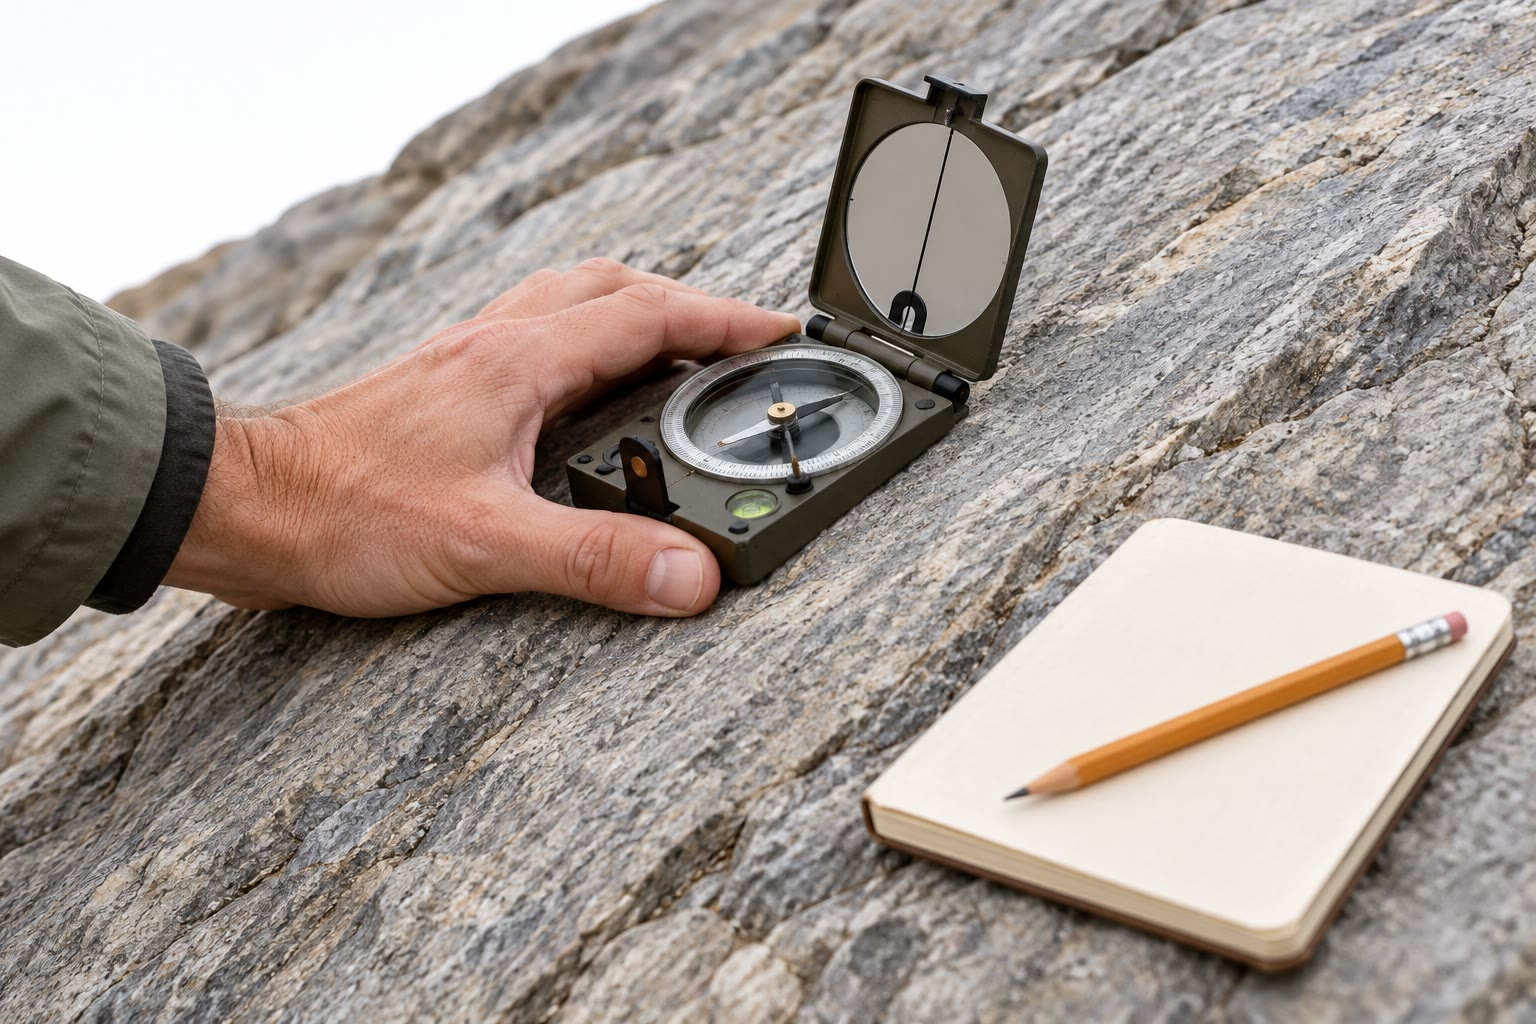
\includegraphics[width=\linewidth]{images/book5/ai/b3-compass-clinometer.jpg}

{\scriptsize A compass-clinometer laid against an inclined rock surface, with a
field notebook (AI-generated illustration).}
\end{minipage}
\end{inthefield}

\section{Exercises}

\begin{exercise}[$\star$]\label{exo:b3:structural-analysis:1}
Give the trend and plunge of the \omterm{def:b3:structural-analysis:stereo}{pole} of the plane $040/30$ (dip direction,
dip). Give the attitude of the plane whose \omterm{def:b3:structural-analysis:stereo}{pole} trends \ang{315} and plunges
\ang{20}.
\end{exercise}

\begin{exercise}[$\star$]\label{exo:b3:structural-analysis:2}
A line plunges \ang{30}. At what distance from the centre does it plot on an
\omterm{def:b3:structural-analysis:stereo}{equal-angle net} and on an equal-area net, both of radius \qty{10}{cm}?
\end{exercise}

\begin{exercise}[$\star$]\label{exo:b3:structural-analysis:3}
The limbs of a fold have the attitudes $090/30$ and $270/30$. Compute the
angle between their \omterm{def:b3:structural-analysis:stereo}{poles} with the dot product of the normals, the interlimb
angle, and the class of the fold.
\end{exercise}

\begin{exercise}[$\star$]\label{exo:b3:structural-analysis:4}
A fault $090/60$ carries striations of rake \ang{-45}. With the strike vector
$\vec s = (0, 1, 0)$ and the down-dip vector $\vec d$ of the plane, the slip
of the hanging wall is $\vec u = \cos r\,\vec s - \sin r\,\vec d$. Compute
$\vec d$, $\vec u$, and the trend and plunge of the slip. Name the fault.
\end{exercise}

\begin{exercise}[$\star\star$]\label{exo:b3:structural-analysis:5}
The limbs of a fold have the attitudes $060/40$ and $250/30$. Compute the
trend and plunge of its axis, and its interlimb angle.
\end{exercise}

\begin{exercise}[$\star\star$]\label{exo:b3:structural-analysis:6}
Compute the fraction of the area of the net that lies inside the circle of
lines plunging more than \ang{60}, on the equal-area and on the \omterm{def:b3:structural-analysis:stereo}{equal-angle
net}, and the fraction of the directions of the lower hemisphere that plunge
more than \ang{60}. Which net should be used to count \omterm{def:b3:structural-analysis:stereo}{poles}?
\end{exercise}

\begin{exercise}[$\star\star$]\label{exo:b3:structural-analysis:7}
Three \omterm{def:b3:structural-analysis:stereo}{poles} lie in the vertical east--west plane, at \ang{-20}, $0$ and
\ang{20} from the vertical: $\vec p = (\sin a, 0, -\cos a)$. Compute their
\omterm{def:b3:structural-analysis:orientation-tensor}{orientation tensor}, its eigenvalues and eigenvectors, and the \omterm{def:b3:structural-analysis:pi}{beta-axis}. Why
is the smallest eigenvalue exactly zero?
\end{exercise}

\begin{exercise}[$\star\star$]\label{exo:b3:structural-analysis:8}
Place on the Flinn diagram the ellipsoid $X : Y : Z = 3 : 1.5 : 1$, then the
ellipsoid of constant volume with $X = 1.8$ and $Y = 1.1$. Compute $k$ for
each and name the strain.
\end{exercise}

\begin{exercise}[$\star\star$]\label{exo:b3:structural-analysis:9}
In a section cut parallel to the stretching, initially round ooids are
ellipses of axial ratio $2.25$, all parallel, and the area of each is
unchanged. Compute the principal stretches and the extension along the long
axis. Before the strain, the ooid centres were never closer than
\qty{0.4}{mm}: give the semi-axes of the void of the Fry plot.
\end{exercise}

\begin{exercise}[$\star\star\star$]\label{exo:b3:structural-analysis:10}
At $\theta = \ang{60}$ from the nadir, compute the stretch along the radius,
$\mathrm dr/(R\,\mathrm d\theta)$, and around the circle, $r/(R\sin\theta)$,
for both projections. Check the theorem on the projections, and give the ratio
of the axes of the oval into which the equal-area net turns a very small
circle there.
\end{exercise}

\begin{exercise}[$\star\star\star$]\label{exo:b3:structural-analysis:11}
In a strike-slip regime, $\sigma_1$ is horizontal towards \ang{000},
$\sigma_3$ horizontal towards \ang{090} and $\sigma_2$ vertical. A vertical
fault strikes \ang{020}. Without computing $\vec\tau$, show that its slip is
horizontal for every $\Phi$. Then compute $-\vec\tau$ for $\Phi = 0.4$ with
the plane's normal $\vec n = (\cos\ang{20}, -\sin\ang{20}, 0)$ and give the
sense of slip.
\end{exercise}

\begin{exercise}[$\star\star\star$]\label{exo:b3:structural-analysis:12}
A section \qty{20}{km} long crosses a train of detachment folds. Two horizons
\qty{1.0}{km} apart stand above their original levels by the areas
\qty{6.0}{km^2} (lower) and \qty{7.5}{km^2} (upper). Compute the shortening,
the depth of the detachment below the lower horizon, the original length of
the section and its relative change of length.
\end{exercise}

\section{Problem: Folds and Faults of the Varden Hills}

\begin{problem}[{Weekend problem --- the axis of a fold, the stress of a fault
set and the restoration of a section, in an invented region}]
\label{pb:b3:structural-analysis:1}
% values: calc/ch08.py; figdata/bachelor-3/stereonet.py (data invented from region.py)
In the Varden Hills, the series' invented region, a Mesozoic cover rests on a
basement of schist and granite. The cover is folded into an upright
anticline and syncline with straight limbs, then cut by a normal fault. A
geologist measured twelve bedding planes on the two limbs of the anticline
(dip direction/dip, in degrees):

\begin{center}
\small
\begin{tabular}{l|cccccc}
\hline
east limb & 075/13 & 084/11 & 089/13 & 079/14 & 086/12 & 072/11 \\
west limb & 283/11 & 272/13 & 281/14 & 288/10 & 276/13 & 274/12 \\
\hline
\end{tabular}
\end{center}

The sums of the upward unit normals of the six readings of each limb are
$\vec S_E = (1.2583, 0.2017, 5.8604)$ and $\vec S_W = (-1.2445, 0.1886,
5.8636)$ (east, north, up). Five faults carry striations (dip direction/dip,
rake of the hanging wall's slip): $120/60/{-90}$ (the main fault), $150/55/{-76}$,
$090/65/{-108}$, $200/70/{-78}$ and $060/50/{-105}$. The main fault has a
throw of \qty{200}{m}. The anticline and syncline axes are \qty{4}{km} apart,
so that the folds repeat every \qty{8}{km} from east to west.

\medskip\noindent\textbf{Part I --- Poles and the beta-axis.}
\begin{enumerate}
  \item Give the trend and plunge of the \omterm{def:b3:structural-analysis:stereo}{pole} of the reading $075/13$, and
        its distance from the centre of an equal-area net of radius
        \qty{10}{cm}.
  \item Compute the upward unit normal of the reading $075/13$; check it
        against $\vec S_E$ in size.
  \item Compute the mean attitude of each limb from $\vec S_E$ and $\vec S_W$,
        the mean resultant lengths, and the root-mean-square scatter of the
        readings about their means.
  \item Compute $\vec S_E\times\vec S_W$, and the trend and plunge of the
        \omterm{def:b3:structural-analysis:pi}{beta-axis}.
  \item Compute the angle between the two mean normals, the interlimb angle,
        and the class of the fold.
  \item The axial plane of this symmetric fold contains the \omterm{def:b3:structural-analysis:pi}{beta-axis} and is
        perpendicular to $\vec m_E - \vec m_W$, the difference of the mean unit
        normals. Give its attitude; is the fold upright?
  \item Give the attitude of the $\pi$-girdle, and say why the \omterm{def:b3:structural-analysis:stereo}{poles} lie on
        it.
\end{enumerate}

\medskip\noindent\textbf{Part II --- The orientation tensor.}
The \omterm{def:b3:structural-analysis:orientation-tensor}{orientation tensor} of the twelve \omterm{def:b3:structural-analysis:stereo}{poles} is
\[
  T = \begin{pmatrix} 0.04400 & 0.00035 & 0.00109\\ 0.00035 & 0.00144 & 0.03179\\
  0.00109 & 0.03179 & 0.95456 \end{pmatrix},
\]
with the eigenvalues $0.95562$, $0.04400$ and $0.00038$.
\begin{enumerate}[resume]
  \item Check that the trace of $T$ is 1. With $\vec b = (0.0053, -0.9994,
        0.0333)$, the unit vector along $\vec S_E\times\vec S_W$, compute
        $\vec b^{\mathsf T}T\vec b$. What does the result say about $\vec b$?
  \item Compute the root-mean-square angle between the \omterm{def:b3:structural-analysis:stereo}{poles} and the girdle.
  \item Explain the value of $\lambda_2$ from the dips of the limbs.
  \item Is the fold cylindrical within the precision of the readings?
  \item The plunge of the \omterm{def:b3:structural-analysis:pi}{beta-axis} is set by the north--south tilt of the
        girdle, to which each \omterm{def:b3:structural-analysis:stereo}{pole} contributes with the scatter found in
        question 9. Estimate the standard error of the plunge.
\end{enumerate}

\medskip\noindent\textbf{Part III --- The palaeostress.}
\begin{enumerate}[resume]
  \item What kind of fault is the main fault? Following Anderson, give the
        directions of $\sigma_1$, $\sigma_2$ and $\sigma_3$.
  \item Show, with the theorem on the slip direction, that the main fault
        slips straight down its dip for every value of $\Phi$. What does it
        tell of $\Phi$?
  \item For the fault $150/55$, compute $\vec n$ and its components $n_1 =
        \vec n\cdot\vec e_1$ and $n_2 = \vec n\cdot\vec e_2$, with $\vec e_1$
        vertical and $\vec e_2$ horizontal towards \ang{030}.
  \item Its slip gives $\vec w = \vec n\times\vec u = (0.771, 0.605, 0.198)$.
        Compute $\Phi$.
  \item The other three small faults give $\Phi = 0.294$, $0.301$ and
        $0.306$. Give the mean, and say where the spread comes from.
  \item What does $\Phi = 0.3$ say of $\sigma_2$?
  \item Compute the P and T axes of the main fault (at \ang{45} from the
        plane, in its dip plane), and compare them with $\sigma_1$ and
        $\sigma_3$.
\end{enumerate}

\medskip\noindent\textbf{Part IV --- Restoring an east--west section.}
\begin{enumerate}[resume]
  \item Compute the apparent dip of the east limb, $080.9/12.3$, on an
        east--west section.
  \item Taking the limbs at \ang{12} on the section, compute the restored
        length of one fold wavelength, the shortening and the relative change
        of length.
  \item Compute the height of the anticline crest above the synclines and the
        excess area of one wavelength, assuming that the synclines stayed at
        the original level.
  \item Compute the depth of the detachment beneath the folded bed. Can the
        folds be detached at the base of the cover, a few hundred metres
        down?
  \item Compute the heave and the slip of the main fault on a section along
        \ang{120}.
  \item On the east--west section, compute the apparent dip of the fault and
        its apparent heave. Which section should be restored?
  \item In what order are the fault and the folds restored, and where are the
        \omterm{def:b3:structural-analysis:restoration}{pin lines} placed?
  \item What is the plunge of the Varden fold axis, recovered from the twelve
        readings?
\end{enumerate}
\end{problem}
